\chapter{Избегаем антипаттернов}

Из этой книги вы узнали о лучших практиках создания React приложений. В первых главах мы познакомились с самыми основами, а затем перешли к более продвинутым подходам.

Вы уже должны уметь создавать переиспользуемые компоненты, объединять их в более сложные структуры и оптимизировать для достижения максимальной производительности. Однако, разработчики тоже люди, которые совершают ошибки. В данной главе мы поговорим о самых распространенных антипаттернах, которых следует избегать.

Изучение распространенных ошибок поможет не только избежать их в будущем, но также увеличить понимание того, как работает React. Для каждой проблемы мы подберем пример, который поможет воспроизвести и исправить ошибку.

В этой главе мы разберем следующие пункты:

\begin{itemize}
  \item Ошибки, связанные с инициализацией состояния компонента при помощи его параметров
  \item Почему не стоит мутировать состояние, и как это влияет на производительность
  \item Как правильно выбрать ключи, чтобы помочь процессу согласования
  \item Почему не стоит передавать все параметры через спред оператор в DOM элементы, и что делать вместо этого
\end{itemize}


\section{Инициализация состояния из параметров}

В этой части мы посмотрим, почему использование параметров, переданных родительским компонентом, для инициализации начального состояния в большинстве случаев является антипаттерном. Я использую слово \textit{большинстве}, потому что даже с полным осознанием происходящего мы можем решить его использовать.

Рассмотрим данную проблему на конкретном куске кода. Начнем с компонента, в которому будет одна кнопка \textit{+} для увеличения значения счетчика.

Создадим компонент на основе класса:

\begin{lstlisting}
class Counter extends React.Component
\end{lstlisting}

В конструкторе определим начальное состояние счетчика значением, пришедшим в параметрах, а также привяжем обработчики событий:

\begin{lstlisting}
constructor(props) {
  super(props)
  
  this.state = {
    count: props.count,
  }
  
  this.handleClick = this.handleClick.bind(this)
}
\end{lstlisting}

Реализация обработчика нажатий очень проста: прибавляем $1$ к текущему значению и сохраняем в состояние.

\begin{lstlisting}
 handleClick() {
  this.setState({
    count: this.state.count + 1,
  })
}
\end{lstlisting}

И в конце, в методе \textit{render}, мы отображаем текущее значение и кнопку для его увеличения:

\begin{lstlisting}
render() {
  return (
    <div>
      {this.state.count}
      <button onClick={this.handleClick}>+</button>
    </div>
  )
}
\end{lstlisting}

Теперь мы можем его отрисовать и передать начальное значение (например $1$) через параметр \textit{count}:

\begin{lstlisting}
<Counter count={1} />
\end{lstlisting}

Все работает в соответствии с нашими ожиданиями: каждое нажатие по кнопке \textit{+} увеличивает текущее значение. Самое время задать вопрос, и в чем же тут проблема?

Есть две главных ошибки:

\begin{itemize}
  \item у нас есть два источника правды (source of truth)
  \item Изменение значения в параметрах никак не повлияет на значение внутри состояния
\end{itemize}

Если мы посмотрим на компонент \textit{Counter} через React Developer Tools, то увидим, что \textit{Props} и \textit{State} содержат похожее значение:

\begin{lstlisting}
    <Counter>
    Props
      count: 1
    State
      count: 1
\end{lstlisting}

Это может начать создавать путаницу относительно того, какое из значений как использовать, какое отображать пользователю и зачем в принципе два одинаковых значения.

А после нажатия на \textit{+} эти значения начинают еще и расходиться в разные стороны:

\begin{lstlisting}
    <Counter>
    Props
      count: 1
    State
      count: 2
\end{lstlisting}

На данный момент можно предположить, что значение внутри состояния отображает актуальное значение счетчика, но в общем случае это не очевидно, и любое изменение компонента может привести к искажению логики или передаче неверных данных дочерним компонентам.

Вторая проблема появляется из-за особенностей работы React с компонентами, а точнее из-за того, что конструктор класса вызывается один раз в момент создания экземпляра класса.

В компоненте \textit{Counter} мы читаем значение параметра \textit{count} и сохраняем его внутрь состояния. И если значение этого параметра изменится (например на $10$), значение внутри компонента все равно останется прежним, так как конструктор уже был вызван один раз и больше вызываться не будет (прим.пер. если компонент не будет полностью перерисован конечно). Это приводит к неконсистентности данных, что как минимум не оптимально и может затруднять отладку.

Но что если мы все-таки хотим использовать значение из параметров для инициализации счетчика и знаем, что значение этого параметра никогда не поменяется?

В этом случае лучшим решением будет явно указать, что это начальное значение, которые бесполезно менять. В качестве решения можно переименовать параметр из \textit{count} в \textit{initialCount}. Тогда нам нужно будет поправить компонент следующим образом:

\begin{lstlisting}
constructor(props) {
  super(props)
  
  this.state = {
    count: props.initialCount,
  }
  
  this.handleClick = this.handleClick.bind(this)
}
\end{lstlisting}

И, соответственно, компонент можно будет использовать следующим образом:

\begin{lstlisting}
<Counter initialCount={1} />
\end{lstlisting}

Теперь достаточно очевидно, что родительский компонент может указать начальное значение счетчика, но не может влиять на его значение в дальнейшем.

\section{Мутирование состояния}

В React из коробки есть простой и понятный способ изменения состояние компонентов. Вы должны использовать функцию \textit{setState}, чтобы сказать библиотеке, как должно измениться состояние конкретного компонента. После обновления состояние, React перерисовывает компонент, после чего у нас снова есть доступ к обновленному состоянию через \textit{this.state}. Все, ничего выдумывать не надо.

Однако, все мы совершаем ошибки и в какой-то момент можем написать код, который будет редактировать состояние напрямую, что приведет к проблемам консистентности данных и производительности.

Если мы мутируем состояние не через функцию \textit{setState}, то могут произойти следующие неприятности:

\begin{itemize}
  \item Компонент не перерисовывается после изменения состояния
  \item После следующего вызова \textit{setState} применятся изменения, записанные напрямую
\end{itemize}

Если мы вернемся к счетчику и изменим обработчик нажатий на следующий:

\begin{lstlisting}
handleClick() {
  this.state.count++
}
\end{lstlisting}

То увидим, что при нажатии на кнопку \textit{+} значение счетчика на экране перестало изменяться. Однако, если мы откроем React Developer Tools, то увидим, что состояние компонента при этом вполне себе меняется. Таким образом мы получили ситуацию, когда данные на экране расходятся с данными внутри компонента. Мало вероятно, что это то поведение, которого вы желаете от компонента.

Если вы допустили такую ошибку в коде, вы можете легко ее поправить при помощи \textit{setState}; но если вы делаете это специально, чтобы избежать перерисовки компонента, скорее всего вам нужно переосмыслить структуру компонента.

Мы уже обсуждали в Главе 3, что единственной причиной хранения данных внутри \textit{state}, может быть потребность этих данных в методе \textit{render}.

Вторая проблема, которая возникает из-за прямой записи изменений в состояние компонента, заключается в том, что эти данные будут применяться непредсказуемо после вызова любого метода \textit{setState} в других компонентах.

Например, если мы немного поправим уже знакомый нам счетчик и добавим в него дополнительную кнопку, по нажатию на которою в состояние компонента будет добавляться новое поле \textit{foo}:

\begin{lstlisting}
<button onClick={() => this.setState({ foo: 'bar' })}>
  Update
</button>
\end{lstlisting}

То мы увидим, что нажатие на кнопку \textit{+} также не будет создавать видимых изменений в работе приложения, но по нажатию на кнопку \textit{Update} значение счетчика будет перепрыгивать сразу на актуальное значение.

Само собой мы хотим избежать такого неконтролируемого поведения.

Помимо проблем с неконсистентностью данных прямое редактирование состояния сказывается не лучшим образом на производительности. Для того, чтобы продемонстрировать это, создадим компонент \textit{List}, похожий на тот, который мы создавали в Главе 9 для знакомства с ключами и \textit{PureComponent}.

Прямое изменение состояния компонента делит на ноль всю пользу от использования \textit{PureComponent}. Давайте создадим компонент \textit{List}, чтобы продемонстрировать это:

\begin{lstlisting}
class List extends React.PureComponent
\end{lstlisting}

Внутри конструктора создадим начальное состояние, содержащее список с двумя элементами, а также привяжем обработчик событий к экземпляру класса:

\begin{lstlisting}
constructor(props) {
  super(props)
  
  this.state = {
    items: ['foo', 'bar'],
  }
  
  this.handleClick = this.handleClick.bind(this)
}
\end{lstlisting}

Обработчик нажатий достаточно прост: в список элементов внутри компонента напрямую добавляется еще один (мы еще увидим, почему так делать не нужно), а затем тот же самый список передается в метод \textit{setState}, чтобы вызвать перерисовку компонента:

\begin{lstlisting}
handleClick() {
  this.state.items.push('baz')
  
  this.setState({
    items: this.state.items,
  })
}
\end{lstlisting}

И в конце компонента идет метод \textit{render}, в котором мы отображаем количество элементов и кнопку для вызова обработчика:

\begin{lstlisting}
render() {
  return (
    <div>
      {this.state.items.length}
      <button onClick={this.handleClick}>+</button>
    </div>
  )
}
\end{lstlisting}

На первый взгляд этот код выглядит корректным, но если мы его запустим и нажмем кнопку \textit{+}, то увидим, что значение на экране не обновляется.

Опять же, если мы откроем React Developer Tool, то увидим, что внутреннее состояние компонента меняется, значит сломалась перерисовка:

\begin{lstlisting}
    <List> State
    items: Array[3]
      0: "foo"
      1: "bar"
      2: "baz"
\end{lstlisting}

Проблема возникает из-за того, что мы мутируем массив, который находится внутри состояния компонента, а не создаем новый.

Добавление нового элемента в массив не пересоздает сам массив. А \textit{PureComponent} проверяет, есть ли изменения в параметрах или состоянии, и, если изменений нет, останавливает перерисовку компонента. Так как в данном случае он получает тот же самый массив (в том смысле, что ссылка на массив осталась той же, а проверка выполняется поверхностно), то на этом перерисовка и заканчивается. Это может быть непривычно поначалу, особенно если вы не привыкли работать с неизменяемыми структурами данных.

Основное решение тут, всегда создавать новый объект перед сохранением его внутрь компонента:

\begin{lstlisting}
handleClick() {
  this.setState({
    items: this.state.items.concat('baz'),
  })
}
\end{lstlisting}

Функция \textit{concat}, которая принимает новый элемент и создает новый массив, содержащий все элементы оригинального массива и пришедший элемент. В этом случае \textit{PureComponent} обнаружит изменение состояние и корректно перерисуется.


\section{Использование индексов для ключей}

В Главе 9 мы говорили о производительности и процессе согласования, где разбирали использование ключей (параметра \textit{key} у компонентов) для помощи React с поиском оптимальной стратегии обновления DOM.

Ключ однозначно определяет соответствие между React и DOM элементами. Поэтому библиотека может понять, какие элементы были добавлены, какие удалены, а какие изменены при изменении состояния или параметров. 

Не стоит пренебрегать использование ключей (а чтобы вы не пренебрегали ими эффективнее, React будет сыпать злобными сообщениями в консоль, если вы забыли их где-то добавить). Однако, не всегда достаточно самого факта из использования; иногда выбор значения для ключей может иметь значение. А использование неверных ключей в определенных ситуациях может привести даже к непредсказуемым результатам. Поэтому в данной части мы посмотрим на пример неправильного использования ключей.

Давайте снова создадим компонент \textit{List}:

\begin{lstlisting}
class List extends React.PureComponent
\end{lstlisting}

В конструкторе создаем список из пары объектов в качестве начального состояния и привязываем обработчики событий:

\begin{lstlisting}
constructor(props) {
  super(props)
  
  this.state = {
    items: ['foo', 'bar'],
  }
  
  this.handleClick = this.handleClick.bind(this)
}
\end{lstlisting}

Реализация обработчика будет немного отличаться от предыдущей, так как на этот раз мы хотим добавлять новый элемент не в конец списка, а в начало:

\begin{lstlisting}
handleClick() {
  const items = this.state.items.slice()
  items.unshift('baz')
  
  this.setState({
    items,
  })
}
\end{lstlisting}

И в методе \textit{render} мы отрисовываем весь список и кнопку \textit{+} для добавления нового элемента:

\begin{lstlisting}
render() {
  return (
    <div>
      <ul>
        {this.state.items.map((item, index) => (
          <li key={index}>{item}</li>
        ))}
      </ul>
      <button onClick={this.handleClick}>+</button>
    </div>
  )
}
\end{lstlisting}

Если вы запустите данный код в браузере, то вы не увидите никаких проблем: кнопка \textit{+} будет добавлять новый элемент в начало списка в соответствии с нашими ожиданиями. Но давайте проведем небольшой эксперимент.

Добавим рядом с каждым элементом списка поле ввода. Мы будем использовать именно поле ввода, так как внутри него можно редактировать содержимое, что добавит наглядности примеру:

\begin{lstlisting}
render() {
  return (
    <div>
      <ul>
        {this.state.items.map((item, index) => (
          <li key={index}>
            {item}
            <input type="text" />
          </li>
        ))}
      </ul>
      <button onClick={this.handleClick}>+</button>
    </div>
  )
}
\end{lstlisting}

Если мы снова запустим компонент в браузере, скопируем значения элементов списка в поля ввода рядом с ними, а затем нажмем на кнопку \textit{+}, то увидим нечто прекрасное (нет).

Как видно на скриншоте, элемента списка уехали вниз, а поля ввода остались на старых позициях, что привело к тому, что значения полей ввода уже не соответствуют элементам списка.

\begin{center}
  \makebox[\textwidth]{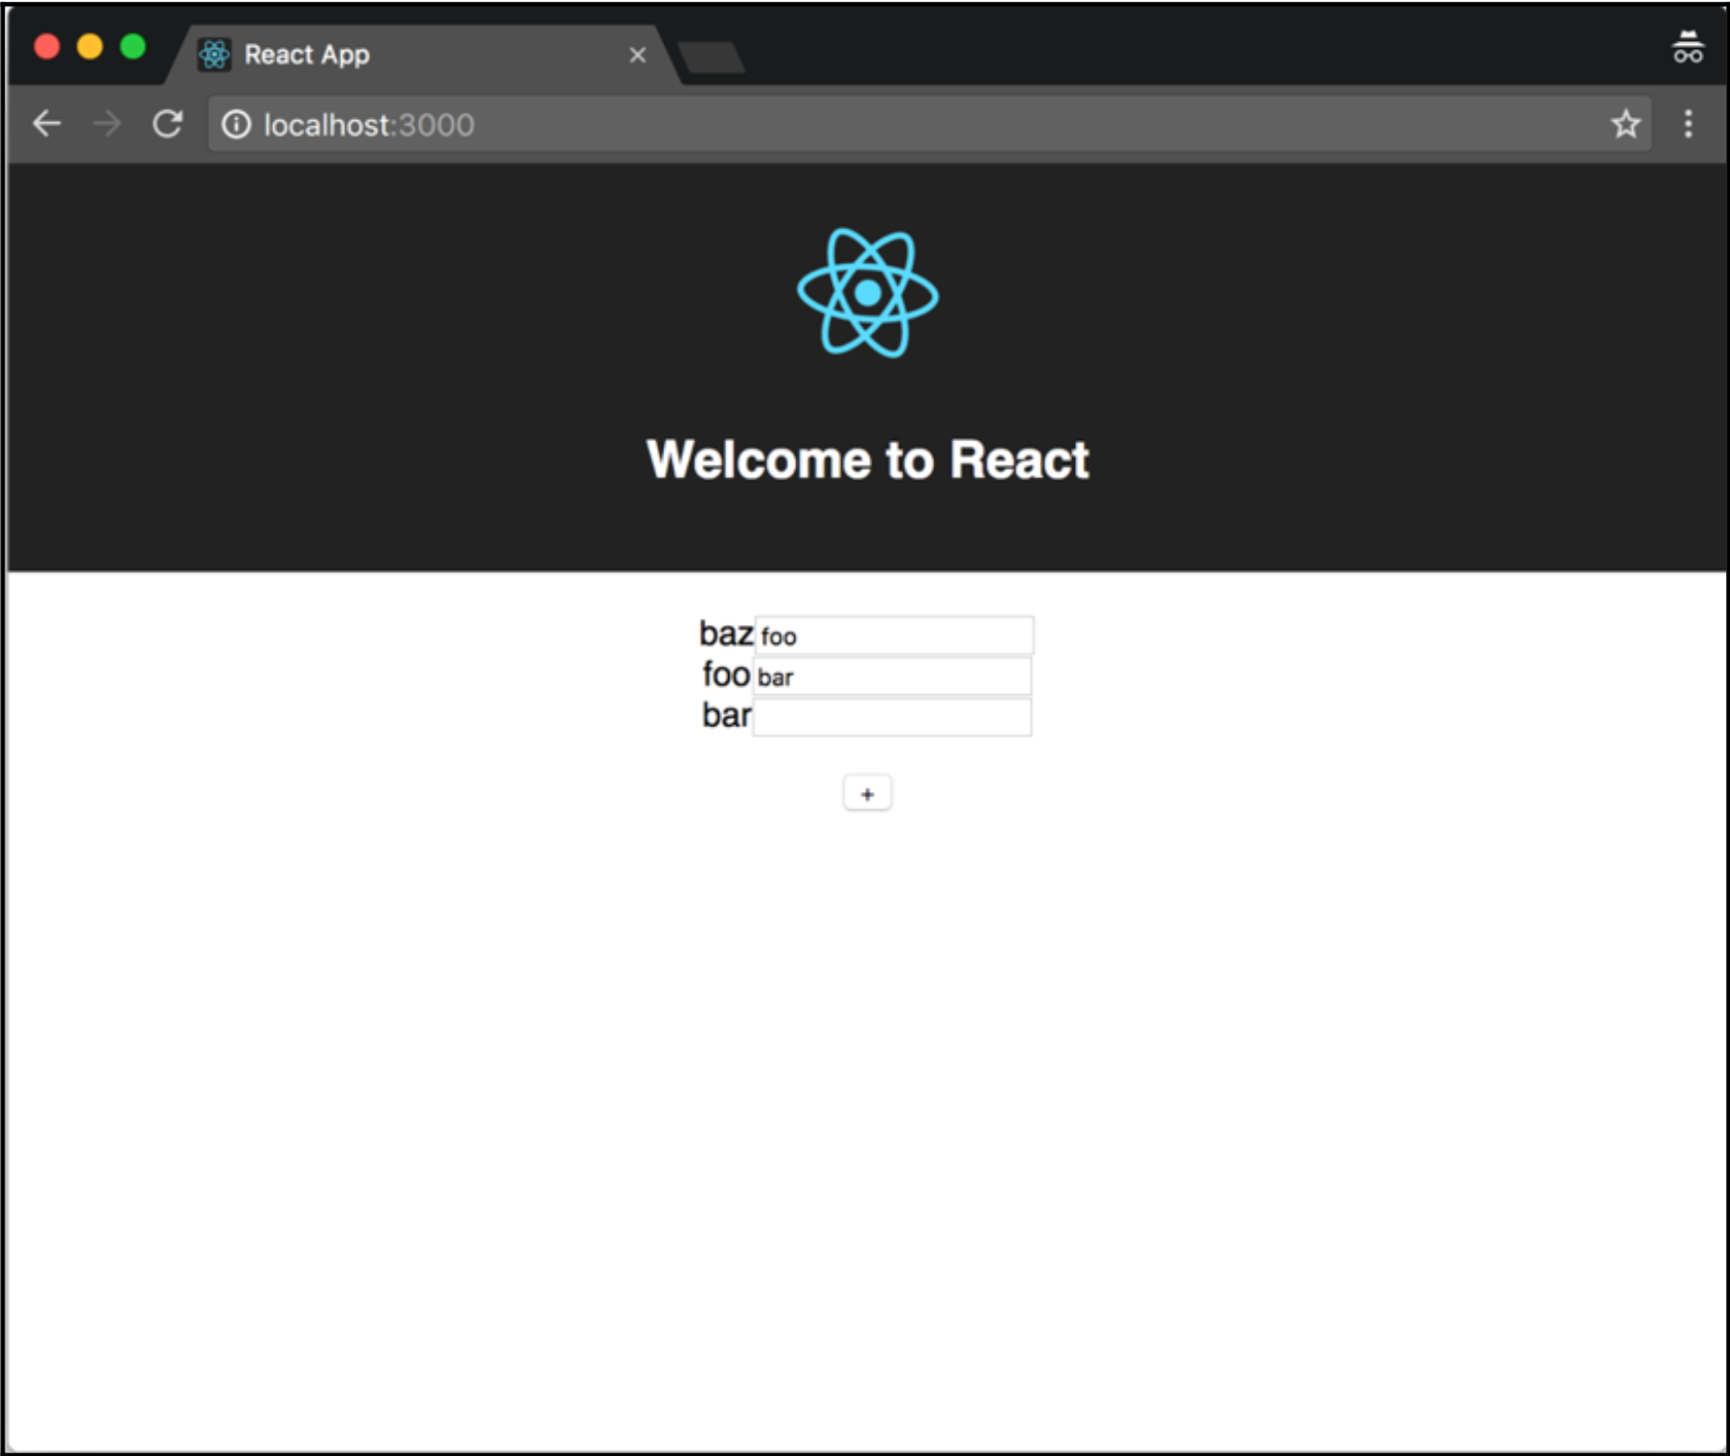
\includegraphics[width=0.6\paperwidth]{images/keys-error}}
\end{center}

Чтобы разобраться и понять, что происходит, мы можем установить \textbf{Perf Add-on}. После установки добавим его в файл с компонентом:

\begin{lstlisting}
import Perf from 'react-addons-perf'
\end{lstlisting}

Мы можем использовать методы жизненного цикла компонента для того, чтобы сохранять информацию о вносимых в DOM изменениях и печатать эту информацию в консоль:

\begin{lstlisting}
componentWillUpdate() {
  Perf.start()
}

componentDidUpdate() {
  Perf.stop()
  Perf.printOperations()
}
\end{lstlisting}

Запуск компонента, нажатие на \textit{+} и проверка консоли принесут нам ответ на эту проблему. 

В консоли мы увидим, что вместо добавления нового элемента в начало списка React сначала меняет текст двух существующих элементов, а затем добавляет новый в конец списка. Это происходит из-за того, что мы используем индексы объектов внутри списка в качестве ключей.

Сложно опровергнуть факт, что индексы элементов массива всегда начинаются с $0$, и добавление нового элемента в начало массива не меняет этого закона мироздания. Поэтому в нашем случае React думает, что мы сначала обновляем два существующих объекта, а затем добавляем новый с ключом (индексом) $2$. Результат такой же, как если бы мы не использовали ключи совсем.

Для решения этой проблемы мы можем использовать значения элементов списка в качестве ключей (если мы уверены, что они не будут повторяться) или мы можем создать для каждого элемента какой-либо уникальный идентификатор.

\section{Спред оператор и параметры DOM элементов}

Есть распространенный подход, который был недавно описан как антипаттерн Деном Абрамовым (\textit{Dan Abramov}); также при использовании этого подхода React выводит страшные предупреждения в консоль.

Этот способ очень часто используется в React сообществе, в чем я неоднократно убеждался на реальных проектах. Мы обычно передаем параметры компоненту через спред оператор, чтобы не передавать каждый в отдельности:

\begin{lstlisting}
<Component {...props} />
\end{lstlisting} 

Данный способ прекрасно работает, а Babel конвертирует его в следующий JavaScript код:

\begin{lstlisting}
React.createElement(Component, props);
\end{lstlisting}

Однако, когда мы передаем параметры DOM элементам таким образом, есть риск, что мы добавим неизвестные для HTML атрибуты, что не является хорошей практикой. 

По сути, проблема даже не в самом спред операторе; мы получим те же самые ошибки и уведомления, если передадим любой не стандартный параметр явным образом. Но из-за того, что спред оператор \textit{скрывает} одиночные параметры, усложняется поиск проблемных мест и конкретных, затесавшихся в DOM параметров.

Для того, чтобы получить уведомления в консоли, о котором мы говорим, достаточно отрисовать следующий компонент:

\begin{lstlisting}
const Spread = () =>  <div foo="bar" />
\end{lstlisting}

И получить примерно следующее сообщение:

\begin{quotation}
Unknown prop `foo` on <div> tag. Remove this prop from the element
\end{quotation}

Сообщение говорит о том, что не следует передавать параметр \textit{foo} элементу \textit{div}.

В данном случае легко найти, какой атрибут должен быть удален, но если мы используем спред оператор следующим образом:

\begin{lstlisting}
const Spread = props => <div {...props} />	
\end{lstlisting}

Мы не можем контролировать параметры, пришедшие из родительского компонента.

Если мы используем этот компонент следующим образом:

\begin{lstlisting}
<Spread className="foo" />
\end{lstlisting}

То никаких проблем нет.

Но если мы сделаем что-то вида:

\begin{lstlisting}
<Spread foo="bar" className="baz" />
\end{lstlisting}

React начнет ругаться, так как мы применяем не стандартный атрибут к DOM элементу.

Одно из решений проблемы -- добавить новый параметр \textbf{domProps}, который мы сможем без опасений передавать в DOM элементы через спред оператор, так как явно указываем, что он содержит только валидные DOM параметры.

Например, мы можем изменить компонент \textit{Spread} следующим образом:

\begin{lstlisting}
const Spread = props => <div {...props.domProps} />
\end{lstlisting}

И использовать его следующим образом:

\begin{lstlisting}
<Spread foo="bar" domProps={{ className: 'baz' }} />
\end{lstlisting}

Как мы уже видели множество раз, в React хорошей практикой является использование явных конструкций.

\section{Заключение}

Знание хороших практик обязательно для написания качественного кода, но иногда, знание об антипаттернах также может уберечь вас от ухода с верного пути. Помимо этого, изучение причин возникновения плохих практик может помочь улучшить понимание работы React.

В этой главе мы рассмотрели 4 подхода использования компонентов, которые могут сломать поведение или ухудшить производительность нашего приложения.

Для каждого из них мы привели пример, который поможет в воспроизведении проблемы, а также способ ее решения.

Мы изучили, почему использование параметров для инициализации состояния может привести к неконсистентности данных, а также посмотрели, почему мутирование состояния компонентов может привести к ухудшению производительности. Также мы разобрались, почему использование неправильных ключей плохо сказывается на процессе согласования, и почему передача параметров DOM элементам через спред оператор является антипаттерном.









